\documentclass[12pt, titlepage]{article}

\usepackage{fullpage}
\usepackage[round]{natbib}
\usepackage{multirow}
\usepackage{booktabs}
\usepackage{tabularx}
\usepackage{graphicx}
\usepackage{float}
\usepackage{hyperref}
\hypersetup{
    colorlinks,
    citecolor=blue,
    filecolor=black,
    linkcolor=red,
    urlcolor=blue
}

%% Comments

\usepackage{color}

\newif\ifcomments\commentstrue %displays comments
%\newif\ifcomments\commentsfalse %so that comments do not display

\ifcomments
\newcommand{\authornote}[3]{\textcolor{#1}{[#3 ---#2]}}
\newcommand{\todo}[1]{\textcolor{red}{[TODO: #1]}}
\else
\newcommand{\authornote}[3]{}
\newcommand{\todo}[1]{}
\fi

\newcommand{\wss}[1]{\authornote{blue}{SS}{#1}} 
\newcommand{\plt}[1]{\authornote{magenta}{TPLT}{#1}} %For explanation of the template
\newcommand{\an}[1]{\authornote{cyan}{Author}{#1}}

%% Common Parts

\newcommand{\progname}{ProgName} % PUT YOUR PROGRAM NAME HERE
\newcommand{\authname}{Team \#, Team Name
\\ Student 1 name
\\ Student 2 name
\\ Student 3 name
\\ Student 4 name} % AUTHOR NAMES                  

\usepackage{hyperref}
    \hypersetup{colorlinks=true, linkcolor=blue, citecolor=blue, filecolor=blue,
                urlcolor=blue, unicode=false}
    \urlstyle{same}
                                


\newcounter{acnum}
\newcommand{\actheacnum}{AC\theacnum}
\newcommand{\acref}[1]{AC\ref{#1}}

\newcounter{ucnum}
\newcommand{\uctheucnum}{UC\theucnum}
\newcommand{\uref}[1]{UC\ref{#1}}

\newcounter{mnum}
\newcommand{\mthemnum}{M\themnum}
\newcommand{\mref}[1]{M\ref{#1}}

\begin{document}

\title{Module Guide for ANN (Artificial Neural Newcounter)} 
\author{Tanya Djavaherpour}
\date{\today}

\maketitle

\pagenumbering{roman}

\section{Revision History}

\begin{tabularx}{\textwidth}{p{3cm}p{2cm}X}
\toprule {\bf Date} & {\bf Version} & {\bf Notes}\\
\midrule
Mar. 19, 2024 & 1.0 & Initial Draft\\
Apr. 10, 2024 & 1.1 & Modification According to Implementation\\
% Date 2 & 1.1 & Notes\\
\bottomrule
\end{tabularx}

\newpage

\section{Reference Material}

This section records information for easy reference.

\subsection{Abbreviations and Acronyms}

\renewcommand{\arraystretch}{1.2}
\begin{tabular}{l l} 
  \toprule		
  \textbf{symbol} & \textbf{description}\\
  \midrule 
  AC & Anticipated Change\\
  ANN & Artificial Neural Network\\
  DAG & Directed Acyclic Graph \\
  GUI & Graphical User Interface\\
  M & Module \\
  MG & Module Guide \\
  OS & Operating System \\
  R & Requirement\\
  SC & Scientific Computing \\
  SRS & Software Requirements Specification\\
  % \progname & Explanation of program name\\
  UC & Unlikely Change \\
  % \wss{etc.} & \wss{...}\\
  \bottomrule
\end{tabular}\\

\newpage

\tableofcontents

\listoftables

\listoffigures

\newpage

\pagenumbering{arabic}

\section{Introduction}

Decomposing a system into modules is a commonly accepted approach to developing
software.  A module is a work assignment for a programmer or programming
team~\citep{ParnasEtAl1984}.  We advocate a decomposition
based on the principle of information hiding~\citep{Parnas1972a}.  This
principle supports design for change, because the ``secrets'' that each module
hides represent likely future changes.  Design for change is valuable in SC,
where modifications are frequent, especially during initial development as the
solution space is explored.  

Our design follows the rules layed out by \citet{ParnasEtAl1984}, as follows:
\begin{itemize}
\item System details that are likely to change independently should be the
  secrets of separate modules.
\item Each data structure is implemented in only one module.
\item Any other program that requires information stored in a module's data
  structures must obtain it by calling access programs belonging to that module.
\end{itemize}

After completing the first stage of the design, the Software Requirements
Specification (SRS) \cite{SRS}, the Module Guide (MG) is developed~\citep{ParnasEtAl1984}. The MG
specifies the modular structure of the system and is intended to allow both
designers and maintainers to easily identify the parts of the software.  The
potential readers of this document are as follows:

\begin{itemize}
\item New project members: This document can be a guide for a new project member
  to easily understand the overall structure and quickly find the
  relevant modules they are searching for.
\item Maintainers: The hierarchical structure of the module guide improves the
  maintainers' understanding when they need to make changes to the system. It is
  important for a maintainer to update the relevant sections of the document
  after changes have been made.
\item Designers: Once the module guide has been written, it can be used to
  check for consistency, feasibility, and flexibility. Designers can verify the
  system in various ways, such as consistency among modules, feasibility of the
  decomposition, and flexibility of the design.
\end{itemize}

The rest of the document is organized as follows. Section
\ref{SecChange} lists the anticipated and unlikely changes of the software
requirements. Section \ref{SecMH} summarizes the module decomposition that
was constructed according to the likely changes. Section \ref{SecConnection}
specifies the connections between the software requirements and the
modules. Section \ref{SecMD} gives a detailed description of the
modules. Section \ref{SecTM} includes two traceability matrices. One checks
the completeness of the design against the requirements provided in the SRS \cite{SRS}. The
other shows the relation between anticipated changes and the modules. Section
\ref{SecUse} describes the use relation between modules.

\section{Anticipated and Unlikely Changes} \label{SecChange}

This section lists possible changes to the system. According to the likeliness
of the change, the possible changes are classified into two
categories. Anticipated changes are listed in Section \ref{SecAchange}, and
unlikely changes are listed in Section \ref{SecUchange}.

\subsection{Anticipated Changes} \label{SecAchange}

Anticipated changes are the source of the information that is to be hidden
inside the modules. Ideally, changing one of the anticipated changes will only
require changing the one module that hides the associated decision. The approach
adapted here is called design for
change.

\begin{description}
\item[\refstepcounter{acnum} \actheacnum \label{acHardware}:] The specific
  hardware on which the software is running.
\item[\refstepcounter{acnum} \actheacnum \label{acInput}:] The format of the
  initial input data.
% \item[\refstepcounter{acnum} \actheacnum \label{acInputSize}:] The constraint on 
%   the size of the input images.
\item[\refstepcounter{acnum} \actheacnum \label{algo}:] Changes in the 
  algorithms and techniques used for image classification.
% \item[\refstepcounter{acnum} \actheacnum \label{methods}:] Evolution of methods 
%   for processing and analyzing input images to extract features.
\item[\refstepcounter{acnum} \actheacnum \label{ANNAlgo}:] Modifications in 
  neural network training algorithms and parameter adjustments.
\item[\refstepcounter{acnum} \actheacnum \label{modelTraining}:] Updates in the 
  scheduling and methodology for model training and updating.
\item[\refstepcounter{acnum} \actheacnum \label{acOutput}:] Evolution in the 
  format and structure of the output data, including classification results, 
  by developing GUI.
\end{description}

\subsection{Unlikely Changes} \label{SecUchange}

The module design should be as general as possible. However, a general system is
more complex. Sometimes this complexity is not necessary. Fixing some design
decisions at the system architecture stage can simplify the software design. If
these decision should later need to be changed, then many parts of the design
will potentially need to be modified. Hence, it is not intended that these
decisions will be changed.

\begin{description}
\item[\refstepcounter{ucnum} \uctheucnum \label{ucIO}:] Input/Output devices
  (Input: File and/or Keyboard, Output: File, Memory, and/or Screen).
\item[\refstepcounter{ucnum} \uctheucnum \label{ucIO}:] The source of input 
  is always external to the software.
\item[\refstepcounter{ucnum} \uctheucnum \label{ucIO}:] The classification results
 (outputs) are always displayed on the output software.
\item[\refstepcounter{ucnum} \uctheucnum \label{ucIO}:] The nature of outputs as 
image classifications is a fixed aspect of the system.
\end{description}

\section{Module Hierarchy} \label{SecMH}

This section provides an overview of the module design. Modules are summarized
in a hierarchy decomposed by secrets in Table \ref{TblMH}. The modules listed
below, which are leaves in the hierarchy tree, are the modules that will
actually be implemented.

\begin{description}
\item [\refstepcounter{mnum} \mthemnum \label{HW}:] Hardware-Hiding Module
\item [\refstepcounter{mnum} \mthemnum \label{ACM}:] ANN Control Module
\item [\refstepcounter{mnum} \mthemnum \label{SavedANN}:] Saved ANN Model Module
\item [\refstepcounter{mnum} \mthemnum \label{Output}:] Output Module
\item [\refstepcounter{mnum} \mthemnum \label{In-class}:] Input Classifier Module
\item [\refstepcounter{mnum} \mthemnum \label{In-set}:] Input Image Module
\item [\refstepcounter{mnum} \mthemnum \label{Train-Model}:] Training Model Module
% \item [\refstepcounter{mnum} \mthemnum \label{Feedback}:] Feedback Module
\item [\refstepcounter{mnum} \mthemnum \label{In-prep}:] Input Preparing and Preprocessing Module
\item [\refstepcounter{mnum} \mthemnum \label{Data}:] Data Preparing and Preprocessing Module
\item [\refstepcounter{mnum} \mthemnum \label{Train}:] Training and Testing Module
% \item [\refstepcounter{mnum} \mthemnum \label{Test}:] Testing Module
\end{description}


\begin{table}[h!]
\centering
\begin{tabular}{p{0.3\textwidth} p{0.6\textwidth}}
\toprule
\textbf{Level 1} & \textbf{Level 2}\\
\midrule

{Hardware-Hiding Module} & ~ \\
\midrule

\multirow{7}{0.3\textwidth}{Behaviour-Hiding Module}
&ANN Control Module\\
&Saved ANN Model Module\\
&Output Module\\
&Input Classifier Module\\
&Input Image Module\\
&Training Model Module\\
% &Feedback Module\\
\midrule

\multirow{3}{0.3\textwidth}{Software Decision Module}
&Input Preparing and Preprocessing Module\\
&Data Preparing and Preprocessing Module\\
&Training and Testing Module\\
% &Testing Module\\

\bottomrule

\end{tabular}
\caption{Module Hierarchy}
\label{TblMH}
\end{table}

\section{Connection Between Requirements and Design} \label{SecConnection}

The design of the system is intended to satisfy the requirements developed in
the SRS \cite{SRS}. In this stage, the system is decomposed into modules. The connection
between requirements and modules is listed in Table~\ref{TblRT}.

% \wss{The intention of this section is to document decisions that are made
%   ``between'' the requirements and the design.  To satisfy some requirements,
%   design decisions need to be made.  Rather than make these decisions implicit,
%   they are explicitly recorded here.  For instance, if a program has security
%   requirements, a specific design decision may be made to satisfy those
%   requirements with a password.}

\section{Module Decomposition} \label{SecMD}

Modules are decomposed according to the principle of ``information hiding''
proposed by \citet{ParnasEtAl1984}. The \emph{Secrets} field in a module
decomposition is a brief statement of the design decision hidden by the
module. The \emph{Services} field specifies \emph{what} the module will do
without documenting \emph{how} to do it. For each module, a suggestion for the
implementing software is given under the \emph{Implemented By} title. If the
entry is \emph{OS}, this means that the module is provided by the operating
system or by standard programming language libraries.  \emph{ANN} means the
module will be implemented by the ANN software.

Only the leaf modules in the hierarchy have to be implemented. If a dash
(\emph{--}) is shown, this means that the module is not a leaf and will not have
to be implemented.

\subsection{Hardware Hiding Modules (\mref{HW})}

\begin{description}
\item[Secrets:]The data structure and algorithm used to implement the virtual
  hardware.
\item[Services:]Serves as a virtual hardware used by the rest of the
  system. This module provides the interface between the hardware and the
  software. So, the system can use it to display outputs or to accept inputs.
\item[Implemented By:] OS
\end{description}

\subsection{Behaviour-Hiding Module}

\begin{description}
\item[Secrets:]The contents of the required behaviours.
\item[Services:]Includes programs that provide externally visible behaviour of
  the system as specified in the software requirements specification (SRS)
  documents \cite{SRS}. This module serves as a communication layer between the
  hardware-hiding module and the software decision module. The programs in this
  module will need to change if there are changes in the SRS \cite{SRS}.
\item[Implemented By:] --
\end{description}

\subsubsection{ANN Control Module (\mref{ACM})}

\begin{description}
\item[Secrets:]The algorithm for coordinating the running of the program.
\item[Services:]Provides the main program.
\item[Implemented By:] ANN
\item[Type of Module:] Abstract Data Type
\end{description}

\subsubsection{Saved ANN Model Module (\mref{SavedANN})}

\begin{description}
  \item[Secrets:]The weights and biases that make up the ANN classification model for th 10
  classes of CIFAR-10 dataset \cite{CIFAR10}.
  \item[Services:]Saves the data of the highest performance model trained by ANN in 
  a .txt file.
  \item[Implemented By:] ANN
  \item[Type of Module:] Record
  \end{description}

\subsubsection{Output Module (\mref{Output})}

\begin{description}
\item[Secrets:]The format and structure of the output data.
\item[Services:]Outputs the class of the uploaded image and receives 
the end user's feedback.
\item[Implemented By:] ANN
\item[Type of Module:] Abstract Object
\end{description}

\subsubsection{Input Classifier Module(\mref{In-class})}

\begin{description}
  \item[Secrets:]The algorithm for classification given the input image and using the 
  saved ANN model.
  \item[Services:]Predicts the class of the uploaded image by getting the saved model from \mref{SavedANN}.
  \item[Implemented By:] ANN
  \item[Type of Module:] Abstract Data Type
\end{description}


\subsubsection{Input Image Module(\mref{In-set})}

\begin{description}
  \item[Secrets:]Receiving the input data.
  \item[Services:]Prompts user for input image and checks its size and format.
  \item[Implemented By:] ANN
  \item[Type of Module:] Abstract Data Type
\end{description}

\subsubsection{Training Model Module(\mref{Train-Model})}

\begin{description}
  \item[Secrets:]The algorithm for implementing the Artificial Neural Network.
  \item[Services:]Provides the architecture and the performance of Artificial Neural Network. 
  This module includes the number of neurons, the connection between them, feedforarding and backpropagassion 
  algorithm.
  \item[Implemented By:] ANN
  \item[Type of Module:] Abstract Data Type
\end{description}

% \subsubsection{Feedback Module(\mref{Feedback})}

% \begin{description}
%   \item[Secrets:]Recording end user's feedback.
%   \item[Services:]Receives the end user's feedback on the classification's accuracy. 
%   This feedback will be used to improve the model's performance and accuracy.
%   \item[Implemented By:] ANN
%   \item[Type of Module:] Record
% \end{description}

\subsection{Software Decision Module}

\begin{description}
\item[Secrets:] The design decision based on mathematical theorems, physical
  facts, or programming considerations. The secrets of this module are
  \emph{not} described in the SRS \cite{SRS}.
\item[Services:] Includes data structure and algorithms used in the system that
  do not provide direct interaction with the user. 
  % Changes in these modules are more likely to be motivated by a desire to
  % improve performance than by externally imposed changes.
\item[Implemented By:] --
\end{description}

\subsubsection{Input Preparing and Preprocessing Module(\mref{In-prep})}

\begin{description}
  \item[Secrets:]Preparing the suitable input data for classifier model
  \item[Services:]Changes the input image form a 3D matrix to an 1D one by grayscaling it and 
  put all the cells next to each other as a vector.
  \item[Implemented By:] ANN
  % \item[Type of Module:] Abstract Data Type
\end{description}

\subsubsection{Data Preparing and Preprocessing Module(\mref{Data})}

\begin{description}
  \item[Secrets:]Preparing the suitable training dataset for model
  \item[Services:]For the better accurate training and testing results, shuffles the training and testing dataset. 
  Changes the traing and test images form 3D matrices to 1D ones by grayscaling them and 
  put all the cells of every image next to each other as vectors.
  \item[Implemented By:] ANN
  % \item[Type of Module:] Abstract Data Type
\end{description}

\subsubsection{Training and Testing Module(\mref{Train})}

\begin{description}
  \item[Secrets:]Finding weights and biases of the model.
  \item[Services:]Applies the training process on prepared trining data from \mref{Data}, using the impelemted model 
  from \mref{Train-Model} to find the best weights between neurons and each neuron's biase. At the same 
  time, tests the model to make sure it is being trained.
  \item[Implemented By:] ANN
  % \item[Type of Module:] Abstract Data Type
\end{description}

% \subsubsection{Testing Module(\mref{Test})}

% \begin{description}
%   \item[Secrets:]Testing the trained model to find the achived accuracy.
%   \item[Services:]Applies the testing process on prepared testing data from \mref{Data}, using the trained model 
%   from \mref{Train} to check the model's merformance.
%   \item[Implemented By:] ANN
%   % \item[Type of Module:] Abstract Data Type
% \end{description}


\section{Traceability Matrix} \label{SecTM}

This section shows two traceability matrices: between the modules and the
requirements and between the modules and the anticipated changes.

% the table should use mref, the requirements should be named, use something
% like fref
\begin{table}[H]
\centering
\begin{tabular}{p{0.2\textwidth} p{0.6\textwidth}}
\toprule
\textbf{Req.} & \textbf{Modules}\\
\midrule
R1 & \mref{HW}, \mref{ACM}, \mref{In-set}, \mref{In-prep}\\
R2 & \mref{ACM}, \mref{Output}, \mref{In-set}\\
R3 & \mref{ACM}, \mref{SavedANN}, \mref{In-class}\\
% R4 & \mref{HW}, \mref{ACM}, \mref{SavedANN}, \mref{Output}\\
% R5 & \mref{ACM}, \mref{Output}\\
\bottomrule
\end{tabular}
\caption{Trace Between Requirements and Modules}
\label{TblRT}
\end{table}

\begin{table}[H]
\centering
\begin{tabular}{p{0.2\textwidth} p{0.6\textwidth}}
\toprule
\textbf{AC} & \textbf{Modules}\\
\midrule
\acref{acHardware} & \mref{HW}\\
\acref{acInput} & \mref{In-set}\\
\acref{algo} & \mref{In-class}\\
\acref{ANNAlgo} & \mref{Train}\\
\acref{modelTraining} & \mref{Train-Model}\\
\acref{acOutput} & \mref{Output}\\
\bottomrule
\end{tabular}
\caption{Trace Between Anticipated Changes and Modules}
\label{TblACT}
\end{table}

\section{Use Hierarchy Between Modules} \label{SecUse}

In this section, the uses hierarchy between modules is
provided. \citet{Parnas1978} said of two programs A and B that A {\em uses} B if
correct execution of B may be necessary for A to complete the task described in
its specification. That is, A {\em uses} B if there exist situations in which
the correct functioning of A depends upon the availability of a correct
implementation of B.  Figure \ref{FigUH} illustrates the use relation between
the modules. It can be seen that the graph is a directed acyclic graph
(DAG). Each level of the hierarchy offers a testable and usable subset of the
system, and modules in the higher level of the hierarchy are essentially simpler
because they use modules from the lower levels.

\begin{figure}[H]
\centering
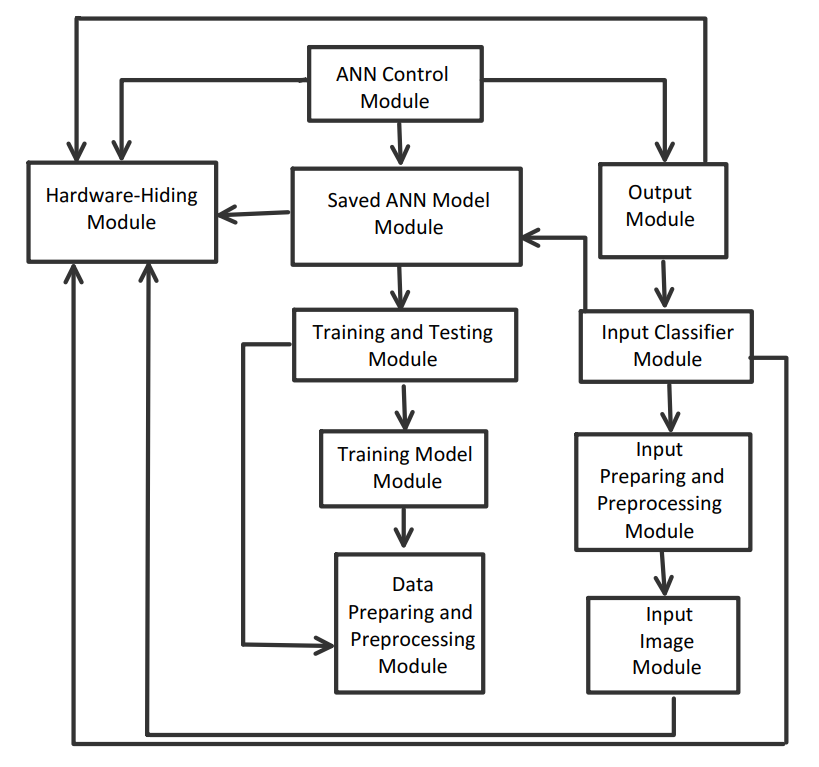
\includegraphics[width=0.7\textwidth]{Modules.PNG}
\caption{Use hierarchy among modules}
\label{FigUH}
\end{figure}

%\section*{References}

% \section{User Interfaces}

% \wss{Design of user interface for software and hardware.  Attach an appendix if
% needed. Drawings, Sketches, Figma}

% \section{Design of Communication Protocols}

% \wss{If appropriate}

% \section{Timeline}

% \wss{Schedule of tasks and who is responsible}

% \wss{You can point to GitHub if this information is included there}

\bibliographystyle {plainnat}
\bibliography{../../../refs/References}

\newpage{}

\end{document}